%% This is file `rinp-template.tex',
%% 
%% Copyright 2016 Elsevier Ltd
%% 
%% This file is part of the 'Elsarticle Bundle'.
%% ---------------------------------------------
%% 
%% It may be distributed under the conditions of the LaTeX Project Public
%% License, either version 1.2 of this license or (at your option) any
%% later version.  The latest version of this license is in
%%    http://www.latex-project.org/lppl.txt
%% and version 1.2 or later is part of all distributions of LaTeX
%% version 1999/12/01 or later.
%% 
%% The list of all files belonging to the 'Elsarticle Bundle' is
%% given in the file `manifest.txt'.
%% 
%% Template article for Elsevier's document class `elsarticle'
%% with harvard style bibliographic references
%%
%% $Id: $
%%
%% Use the option review to obtain double line spacing
%\documentclass[times,review,preprint,authoryear]{elsarticle}

%% Use the options `twocolumn,final' to obtain the final layout
%% Use longtitle option to break abstract to multiple pages if overfull.
%% For Review pdf (With double line spacing)
%\documentclass[times,twocolumn,review]{elsarticle}
%% For abstracts longer than one page.
%\documentclass[times,twocolumn,review,longtitle]{elsarticle}
%% For Review pdf without preprint line
%\documentclass[times,twocolumn,review,nopreprintline]{elsarticle}
%% Final pdf
\documentclass[times,twocolumn,final]{elsarticle}
%%
%\documentclass[times,twocolumn,final,longtitle]{elsarticle}
%%


%% Stylefile to load RINP template
\usepackage{rinp}
\usepackage{framed,multirow}

%% The amssymb package provides various useful mathematical symbols
\usepackage{amssymb}
\usepackage{latexsym}

% Following three lines are needed for this document.
% If you are not loading colors or url, then these are
% not required.
\usepackage{url}
\usepackage{xcolor}
\definecolor{newcolor}{rgb}{.8,.349,.1}

\journal{Public Health}

\begin{document}

\verso{Sayed Ahmed \textit{et al.}}

\begin{frontmatter}

%\title{Type the title of your paper, only capitalize first word and proper nouns\tnoteref{tnote1}}%
\title{Impact of Dietary Recommendations Shift on  Chronic Kidney Disease\tnoteref{tnote1}} 

%\tnotetext[tnote1]{This is an example for title footnote coding.}
%\tnotetext[tnote1]{No research grant is utilized for this research}
%\tnotetext[1]{This document is the results of the major research project done for MSc in the data science and analytics department}
%\tnotetext[2]{No research grant is utilized for this research}

\author[1]{Sayed \snm{Ahmed}\corref{cor1} } %\corref{cor1}
\ead{sayed.ahmed@ryerson.ca}
\ead[url]{ryerson.ca, sayed.ahmed@ryerson.ca}
%\cortext[cor1]{Corresponding author: Tel.: +0-000-000-0000;  fax: +0-000-000-0000;}
  
\author[2]{Youcef \snm{Derbal}\corref{cor2}} %\fnref{fn1}\corref{cor2}
\ead{yderbal@ryerson.ca}
\ead[url]{ryerson.ca, yderbal@ryerson.ca}
%\fntext[fn1]{This is author footnote for second author.}  

%\address[1]{Affiliation 1, Address, City and Postal Code, Country}
\address[1]{Data Science Department, Ryerson University, Toronto, Canada}
%\address[2]{Affiliation 2, Address, City and Postal Code, Country}
\address[2]{Department of Information Technology Management, Ryerson University, Toronto, Canada}

\cortext[cor1]{Corresponding author}
\cortext[cor2]{Principal corresponding author}

\received{1 Sept. 2019}
\finalform{10 Sept 2019}
\accepted{13 Sept. 2019}
\availableonline{15 Oct. 2019}
\communicated{S. Ahmed}

\begin{abstract}
%%%
Chronic Kidney Disease (CKD) leading to End-Stage Renal Disease (ESRD) is very prevalent today. Over 37 millions of Americans have CKD. CKD/ESRD and interrelated diseases cause a majority of the early deaths.  Many research studies have investigated the effects of drugs on CKD. However, less attention has been given to the study of the dietary patterns on CKD progression and mortality. Additionally, recent dietary recommendations shift is not extensively studied for impact on the CKD patients. This research study has uncovered significant correlations between dietary patterns and CKD mortality, also on CKD diagnostic markers such as the Albumin to Creatinine Ratio (ACR). This study also compared the findings with Dietary Recommendations shift for Impact on CKD patients. In this study, Dietary surveys from NHANES, and CKD Mortality dataset from USRDS, Food Grouping datasets from USDA, Shift Recommendation study by CDC were utilized. Principal Component Analysis and Regression were utilized to find the effect on CKD mortality. Grains, Fruits, Alcohols, Nuts showed negative correlations where Vegetables such as Other Vegetables, Starchy Vegetables, and Red and Orange Vegetables showed positive correlations. ACR values were not found strongly correlated with dietary patterns. Comparison with Dietary Recommendations Shift study found that recommended shifts on Fruits, Fats, Polyunsaturated Fats will be beneficial to CKD patients whereas adaptations to reduce harmful effects are required for Vegetables, Whole and Refined Grains.
%%%%
\end{abstract}

\begin{keyword}
%% MSC codes here, in the form: \MSC code \sep code
%% or \MSC[2008] code \sep code (2000 is the default)
%\MSC 41A05\sep 41A10\sep 65D05\sep 65D17
%% Keywords
\KWD CKD  \sep ESRD \sep  Dietary Patterns \sep  Mortality \sep  ACR \sep  Dietary Recommendations Shift
\end{keyword}

\end{frontmatter}

%\linenumbers
%% main text
\section*{Introduction}
\noindent  Chronic kidney disease (CKD) is very prevalent in today’s world and CKD incidents are continually increasing whereby 10 to 13\% of the US population are affected by Chronic Kidney Disease\cite{Jaimonetal2017}. CKD/ESRD and other interrelated diseases such as Hypertension, Heart Diseases, and Diabetes cause the majority of early  deaths \cite{Hannan2019}. In addition to kidney failure, CKD is also a major cause of death from stroke, and heart diseases. On the other hand, hypertension and diabetes are also major causes of CKD. CKD is not reversible, progressive and gradually reduces kidney function. 

\medskip

\noindent Primary causes of CKD include High Blood Pressure, and Diabetes. Other causes include infection, kidney stones, genetics, genetical polycystic kidney disease, certain foods and food habits, pain killers, and drug usage/abuse. As CKDs are neither curable nor reversible controlling diabetes and blood pressure with or without medication can slow the progress of CKDs in most cases. As Kidneys filter waste products and our diet produces those waste products controlling diet have an effect on how much work kidney has to perform, and how well kidneys will function. Studies show that drugs as well as lifestyle choices (food, diet, exercise) can prevent CKD, slow the progression of CKD \cite{Jaceketal2017}, delay dialysis and kidney transplantation; consequently can prevent early deaths. Although there are many studies on the effect of drugs to control CKD and related complications, there are few studies on the effect of diets, dietary patterns, and lifestyles\cite{Jaceketal2017}. There  are studies on how controlling nutrients/chemicals in food items can help to prevent or to slow the progression of CKD. CKD patients are also provided recommendations on certain chemicals or food items. However, adhering to the recommended amount of nutrients and/or food item is challenging. Hence, there is an emerging trend where the effect is studied utilizing  dietary patterns with food groups and food subgroups rather than nutrients/chemicals in food or individual food item. This research analyzes the effect of dietary patterns, using food groups and food subgroups, on  the mortality and survival of CKD patients. Also studied in this research is the correlation between dietary patterns and ACR. 

As Dietary recommendations are difficult to adhere to in food item or nutrient level, there are studies such as by CDC (health.gov) to shift the recommendations in dietary patterns using food groups and subgroups. This study also has explored the dietary recommendations shift by CDC and compared the correlation of Food Groups/Subgroups with CKD Mortality and ACR to understand how the shift recommedation affect CKD patients.

\subsection{How CKD is Identified and Measured}
CKD is identified with one of two measures such as a blood test named Glomerular Filtration Rate (GFR) or a urine test named Albumin to Creatinine Ratio (ACR).  ACR values less than 30 indicates no CKD or mild CKD. ACR values between 30 and 300 indicate moderate CKD. ACR values \textgreater 300 indicates severe CKD. Patients are diagnosed with a CKD disease if the ACR values persist within the above ranges for three months. GFR is measured in ml/min/1.73 m2. CKDs as measured with GFRs are described in stages such as Stage 1 with normal or high GFR (GFR greater than or equal to  90 mL/min), Stage 2 with Mild CKD (GFR = 60-89 mL/min), Stage 3A with Moderate CKD (GFR = 45-59 mL/min), Stage 3B with Moderate CKD (GFR = 30-44 mL/min), Stage 4 with Severe CKD (GFR = 15-29 mL/min), Stage 5 with End Stage CKD (GFR \textless 15 mL/min) \cite{Huangetal2013}. At stage 5, patients loose complete kidney function. At this point, patient survival will require either dialysis or organ transplantation.

\section{Literature Review}

Kidney patients are commonly given dietary advice about intake of individual nutrients, chemicals, food items, or about their whole eating patterns. However, dietary recommendations are challenging to adhere to for the majority of the patients [2]. Also, there is limited evidence that adherence to such advice prevents clinical complications [23]. Hence, studying the whole dietary patterns rather than single nutrient or food group restrictions is an emerging trend for CKD/ ESRD patient diets [2] [24-26]. This is also easier to adhere to. There are several studies on analyzing the relation between dietary patterns and clinical outcomes for CKD patients \cite{Jaceketal2017} \cite{Chenetal2016}  \cite{Gutierreztal2014}   \cite{Huangetal2013}   \cite{Muntneretal2013}  \cite{Ricardoetal2013} \cite{Tsuruyaetal2015}   \cite{Ricardoetal2015} 

\noindent Chen at al \cite{Chenetal2016} studied the association between plant protein intake and mortality in CKD. In the study higher plant protein ratio was found to cause lower mortality for CKD patients in stage 3 or higher ( eGFR  \textless 60 ml/min/1.73 m2 ) though not for others (stage 1 and 2) \cite{Chenetal2016}. This study primarily used statistical methods and Regression Models such as Cox regression models to find the association \cite{Chenetal2016}. Hao-Wen et al [26] studied the association between vegetarian diets and CKD. The study found that vegetarian diets including vegan and ovo-lacto vegetarian diets were possible protective factors. The study utilized The multivariable logistic regression analysis [26].

\noindent Gutiérrez et al \cite{Gutierreztal2014} studied 5 empirically derived dietary patterns such as "convenience" (Chinese and Mexican foods, pizza, and other mixed dishes), "plant-based" (fruits and vegetables), "sweets/fats" (sugary foods), "Southern" (fried foods, organ meats, and sweetened beverages), and "alcohol/salads" (alcohol, green-leafy vegetables, and salad dressing) \cite{Gutierreztal2014}. The study found that dietary pattern rich in processed and fried foods was associated with higher mortality in persons with CKD. On the other hand, a diet rich in fruits and vegetables was found to be protective \cite{Gutierreztal2014}.

\noindent Huang et al. \cite{Huangetal2013} studied whether Mediterranean diet can preserve kidney function along with maintaining favorable cardiometabolic profile with reduced mortality risk for individuals with CKD. The study found that adhering to Mediterranean diet has a lower likelihood of having CKD in elderly men. The study also found that a greater adherence to this diet can improve survival for CKD patients \cite{Huangetal2013}. Huang et al \cite{Huangetal2013} in the above study, used unpaired t test, nonparametric Mann–Whitney test, or chi-square test as appropriate for Comparisons between CKD and non-CKD men. To evaluate the association of Mediterranean diet with the presence of CKD, Crude and multiple adjusted logistic regression models were fitted. All tests were two-tailed, and P \textless 0.05 was considered significant \cite{Huangetal2013}. One aspect of Muntner et al \cite{Muntneretal2013} study was to find out how Life’s Simple 7 factors (Smoke, Activity, BMI, Diet, Blood Pressure, Cholesterol, and Glucose) affect in getting ESRD. For each factor, participants were assigned to one of  three levels of compliance to the recommendations. The three levels are ideal, intermediate, and poor. The study shows that people who have ideal scores in more of these factors have lower likelihood of getting ESRD. This study utilized Cox proportional hazards models. Adjustment were made for age, race, sex, stroke-based geographic region of residence, income, education, and history of stroke or coronary heart disease \cite{Muntneretal2013}.

\noindent  Ricardo et al \cite{Ricardoetal2013} studied the association of death to healthy lifestyles especially in relation to CKD. The study found that adherence to healthy lifestyles was associated with lower risk for mortality in CKD patients. In this study, to determine the association between a healthy lifestyle and survival among individuals with CKD, Cox proportional hazards models were used while also adjusting for important covariates. Stratified survival analyses by eGFR and UACR was performed for Sensitivity analyses \cite{Ricardoetal2013}. Suruya et al. \cite{Tsuruyaetal2015} studied dietary patterns in hemodialysis patients in Japan and researched associations between dietary patterns and clinical outcomes. The study found that patients with unbalanced diet were more likely to have adverse clinical outcomes. Hence, such patients when in addition to portion control, maintains a well-balanced diet especially for the food groups meat, fish, and vegetables will have less adverse clinical outcomes \cite{Tsuruyaetal2015}. Tsuruya et al \cite{Tsuruyaetal2015} utilized a principal components analysis (PCA) with Promax rotation to reduce to a smaller set of food groups for analysis. PCA was used to find food groups eaten with equal frequencies \cite{Tsuruyaetal2015}. Cox regression model was used for the analysis with multiple models where each model had a different combination of covariants \cite{Tsuruyaetal2015}.

\noindent Another study by Ricardo et al \cite{Ricardoetal2015} estimated the degree of adherence to a healthy lifestyle that decreases the risk of renal and cardiovascular events among adults with chronic kidney disease (CKD). The study found that adherence to a healthy lifestyle was associated with lower all-cause mortality risk in CKD. The greatest reduction in all-cause mortality was related to nonsmoking \cite{Ricardoetal2015}. This study by Ricardo et al \cite{Ricardoetal2015}, to compare categorical and continuous variables used Chi-squared and analysis of variance tests respectively. To examine the association between healthy lifestyle and outcomes, Cox proportional hazards models were used. Death was treated as a censoring event. Three nested Cox proportional hazards models were fitted and were adjusted sequentially for potential explanatory variables \cite{Ricardoetal2015}. G. Asghari et al [27] studied the association of population-based dietary pattern with the risk of incident CKD. The study concluded that high fat and high sugar diet pattern is associated with significantly increased (46\%) odds of incident CKD where a lacto-vegetarian diet can be protective of CKD by 43\%. The study utilized multivariable logistic regression to calculate odds ratio for the association.

\noindent  Overall, most of the reviewed studies primarily used direct clinical data of patients for several years and applied statistical analysis primarily. This research primarily utilized public datasets from CDC, USRDS.  One of the studies above utilized the dietary pattern data from CDC and NHANES like this study. However, this study will differ in the methodology, exploration, and analysis. This study is finding relations between datasets from multiple sources and is focused on finding patterns and relations in general population than specific/selected individuals. Most of the studies above utilized primarily statistical methods and sensitivity analysis where primarily regression models especially Cox regression models were used. In a couple of cases, Principal Component Analysis (PCA) was used. This research primarily utilized public datasets from CDC, USRDS, Health.gov. For association and prediction, PCA, Regression, and several machine learning approaches are utilized. For food groups and subgroups,  we utilized the USDA categorization. Recommended amounts for food groups provided by CDC/Health.gov is used. Additionally, ACR values are predicted based on datasets by CDC such as NHANES dietary intake survey, and laboratory data on ACR. For the prediction, machine learning approaches are used.  The machine learning approaches used for ACR value prediction are: Regression and Bayesian.
%\section{Exploratory Study}
Initially Datasets from USRDS on CKD and ESRD patients were explored for Patient characteristics, prevalence of CKD, dietary intake, dietician care, mortality, and survival. Dietary intake data were missing in these datasets, although dietician care data, mortality and survival data by age groups were included. Furthermore, the dataset did not include any linking data for dietician care data, and target mortality/survival data. Hence, datasets from a study on dietary shift recommendation by CDC was explored. These datasets include recommended intake amounts for each age groups including average intake amount (of food groups and food subgroups) by age groups were provided. However, the dietary shift recommendation of the CDC datasets and USRDS mortality i.e. target variable data were not aligned, the dietary intake data from NHANES survey were explored. Hence, NHANES survey data were regrouped to reflect the USRDS age groups, while the USDA codes were used for Food groups/subgroups/intake food for NHANES survey. Finally the USRDS data, combined with the shift recommendation dataset along with additional data from CDC and other sources were explored to create food group recommended amounts for matching age groups. An initial exploratory analysis was performed on the combined datasets using univariate analysis, bivariate analysis, regression, and factor analysis. The results of these explorations are given in Figure  \ref{exploratory-output}.

\begin{table}[!htb]
\caption{\textbf{Regression Output from Exploratory Analysis using Excel (Data Analysis Module)}}
\begin{tabular}{  | p{2cm} | p{2 cm}  | p{2 cm} | }
\hline
   \textbf{Metrics} & \textbf{Food Groups} & \textbf{Food Subgroups} \\
\hline   
   \textbf{Multiple R}	& 0.880156954 & 0.999378722\\
\hline
\textbf{R Square}	& 0.774676264 & 0.99875783\\
\hline
\textbf{Adjusted R Square} &	0.616949648 &  0.978883104\\ 
\hline
\textbf{Standard Error}	& 6.223447127 & 1.461167293\\
\hline
\end{tabular}
\end{table}

\begin{figure}
\begin{tabular}{|c|}
\hline
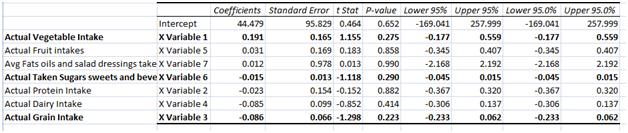
\includegraphics[scale=0.25]{excel-regression-food-groups} \\
\textbf{Regression on Actual Food Group Intake}\\
\hline
\end{tabular}

\begin{tabular}{|c|}
\hline
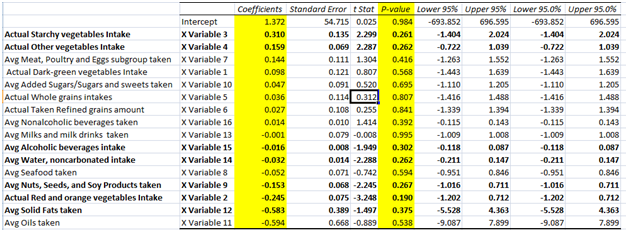
\includegraphics[scale=0.25]{excel-regression-food-subgroups}\\
\textbf{Regression on Actual Food Subgroup Intake} \\
\hline
\end{tabular}

\begin{tabular}{|c|}
\hline
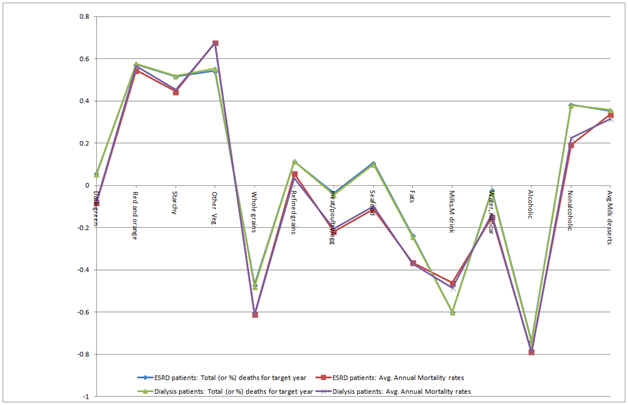
\includegraphics[scale=0.45]{line-plot-regression-exploratory.png}\\
\textbf{Line Plot for Regression outcome}\\
\hline
\end{tabular}

\begin{tabular}{|c|}
\hline
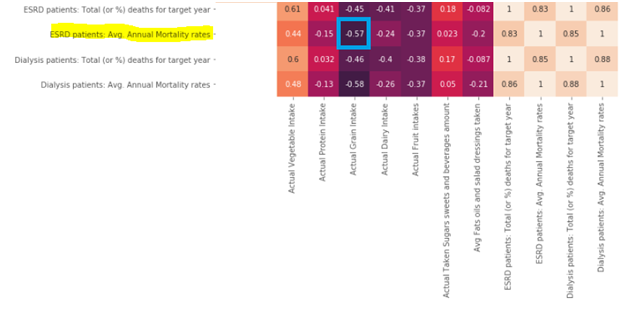
\includegraphics[scale=0.45]{heatmap-exploratory}\\
\textbf{Heatmap for exploration}\\
\hline
\end{tabular}
\caption{\textbf{Exploratory Analysis and Representative Output}}
\label{exploratory-output}
\end{figure}
\section*{Methodology}
The research methodology is summarized by the diagram given in Figure \ref{methodology-new}. 

\begin{figure}
\centering
%\begin{center}
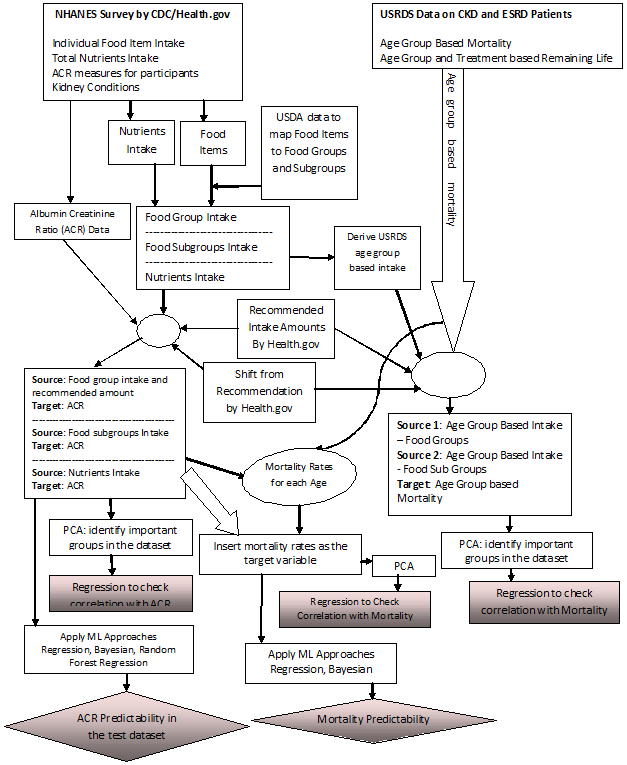
\includegraphics[scale=0.48]{./images/methodologies-enhanced}
%\end{center}
\caption{\textbf{Methodology in a Diagram}}
\label{methodology-new}
\end{figure}

\subsection*{Methodology Overview}
 Dietary survey dataset from NHANES, and age group based CKD Mortality dataset from USRDS, Food Grouping and subgrouping datasets from USDA, Shift Recommendation study by CDC are utilized in this study. NHANES survey dataset by CDC/Health.gov have data with the dietary habits and ACR values for close to 10,000 individuals.  This study utilized Principal Component Analysis to identify the most important food groups and subgroups affecting the ACR value and the CKD Mortality rates.  Statistical regression and factor analysis were then applied to understand the correlation between ACR, and Mortality rates to dietary patterns. We identified important food groups and subgroups that affect ACR and Mortality positively or negatively. The findings were then compared against the Dietray Recommendations shift  \cite{Health2015} by CDC to compare how the recommendations shift affect CKD patients.

\subsection*{Study Selection}
For dietary patterns, CKD measures (such as Albumin to Creatinine Ratio - ACR), and Kidney condition measures, a dataset from the National Health and Nutrition Examination Survey on dietary habits conducted by the CDC \cite{CDC2015} was used. The survey has data from 1996 to 2016 \cite{CDC2015}. This study primarily utilized data for 2015-2016. The survey recorded 24 hours individual food item intake amount. Two surveys were taken within 3 to 10 days apart. Each survey provided food item intake amounts in a day and recorded the diet style as well as diet-restrictions. Individual food items are represented using USDA food code. The survey also provided total nutrients data. CDC also released examination, laboratory, demographics, and other related data for those participants. This study explored and utilized examination data such as Kidney Condition data, laboratory data such as ACR data \& Blood Pressure data, and demographics data for age.
 
For mortality and survival information, dataset from the United States Renal Data System (USRDS) on CKD and ESRD \cite{USRDS2015} \cite{USRDS2018} were utilized. “USRDS investigates the transition of care from CKD to ESRD and end-of-life care for those with advanced kidney disease” \cite{USRDSAnnual2018}. USRDS also releases data on the Incidence, Prevalence, Patient Characteristics, and Treatment Modalities on CKD, and ESRD patients. USRDS  reports survival and mortality using metrics such as Mortality rates, Total Mortality Count,  90 day survival for dialysis and/or transplantation patients,  10 year survival for dialysis and/or transplantation patients, Average Expected remaining lifetime with or without pre-condition and treatment options used.  The data are either aggregated or patient specific detail data. This research utilized only the public dataset i.e. age-group based aggregated data. In couple of experiments, aggregated age-group based data from USRDS was mapped to specific age for NHANES data for each age and participants.

The dietary survey data (NHANES) represented the food items taken by the participants using USDA food codes \cite{ARS2016} \cite{CDC2004} \cite{USDA2010}. Hence, USDA food codes \cite{ARS2016} \cite{CDC2004} \cite{USDA2010} are used to assign food groups and subgroups to the NHANES \cite{CDC2015} survey data to properly group/subgroup the dietary intake of the participants with some customizations.

The shift recommendation study \cite{Health2015}  as part of national act studied the current food habits of U.S. population and identified compliance to provide guidance based on current scientific and medical knowledge. Based on their study, they have recommended areas where adjustments wil be important to the dietary recommendations so that it becomes easier for the people to adhere to the recommendations.  The dietary guidelines provided guidelines that encourage `healthy eating patterns, recognize that individuals will need to make shifts in their food and beverage choices to achieve a healthy pattern, and acknowledge that all segments of our society have a role to play in supporting healthy choices''. These Guidelines also embody the idea that a healthy eating pattern is an adaptable framework in which individuals can enjoy foods that meet their personal, cultural, and traditional preferences while being within their budget. CDC also provided suggestions on how to change the dietary habits. \cite{Health2015}.

\subsection*{Data Synthesis}
NHANES survey data as provided for two days are averaged to get the intake amount for one day. Both individual food item data and nutrients intake data are averaged. USDA food codes are used to map food items to food groups and subgroups. The same food grouping and subgrouping approach utilizing USDA as used by the shift recommendation study is used with negligible exceptions.

ACR and Kidney condition data for each individual are merged with the averaged food groups, subgroups, and nutrients data for the non-age group based studies. This data was further complemented with the food group recommendations data from health.gov, and mortality rate by age from the USRDS. ACR values and mortality rate  are used as the target variables.

In another mortality experiment, the above synthesized datasets were aggregated for USRDS age  groups to calculate average food group/subgroup intake by age groups. 

PCA was applied to find out important food groups and subgroups while regression was applied to find potential associations with ACR and Mortality. 
%\newcommand{\specialcell}[2][c]{%
\begin{tabular}[#1]{@{}l@{}}#2\end{tabular}}
\section{Experiment Design}
\noindent Experiments as provided in Tables \ref{experiment-start} to \ref{experiment-end} are designed to find associations between dietary patterns and CKD mortality as well as to predict ACR values. All of these experiments except set 8 and 9 are conducted.

\begin{center}
\begin{table}[!htb]
\small
\caption{\textbf{Set 1: Association of Food Groups with CKD Mortality}}
\label{experiment-start}
\vspace{0.25cm}
\begin{tabular}{| p{3cm}  |  p {12cm} | }
\hline
\noindent \textbf{Primary Input Dataset:} &  NHANES dietary intake survey aggregated by USRDS age groups to calculate average food item  intake by the participants \\
\hline
\noindent \textbf{Target Variable:} & ESRD: Avg. Annual Mortality rates \\
\hline
\noindent \textbf{Experiment 1.1:}  &   \noindent Identify contributing and important food groups in the dataset  using PCA  a) Using Actual Intake Amount  b) Using ratios of intake and recommended high amounts\\
\hline
\noindent \textbf{Experiment 1.2:}  &  Find correlation (using Pearson’s correlation and regression)  between CKD  mortality and important food groups as found  using PCA  in  experiment 1.1.   a) Using Actual Intake Amount   b) Using ratios of  intake and recommended high amounts \\
\hline
\end{tabular}
\end{table}
\end{center}

\begin{table}[!h]
\caption{\textbf{Set 2: Association of Food Subgroups with CKD Mortality}}
\label{experiment-3}
\vspace{0.25cm}
\begin{tabular}{| p{3cm}  |  p {12cm} | }
\hline
\noindent \textbf{Primary Input Dataset:} &  { NHANES survey aggregated by USRDS  age groups to calculate average food item (food subgroups) intake by the participants  }  \\
\hline
\noindent \textbf{Target Variable:} & ESRD: Avg. Annual Mortality rates \\
\hline
\noindent \textbf{Experiment 2.1:}  & {Identify important food sub groups in the dataset using PCA  and Actual  Average Intake Amount } \\
\hline
\noindent \textbf{Experiment 2.2:}  & {Similar to experiment 1.2 (Regression); however, used food  subgroups  and actual average intake amount only} \\
\hline
\end{tabular}
\end{table}

\begin{table}[!htb]
\caption{\textbf{Set 3: Effect of Food Groups on ACR}}
\label{experiment-4}
\vspace{0.25cm}
\begin{tabular}{| p{3cm}  |  p {12cm} | }
\hline
\noindent \textbf{Primary Input Dataset:} & NHANES survey data for each participant; intake amounts for food groups were averaged for  two surveys. This data was merged with  laboratory tests for ACR \\
\hline
\noindent \textbf{Target Variable:} & Albumin to Creatinine Ratio (ACR) \\
\hline
\noindent \textbf{Experiment 3.1:}  & { Identify contributing and important food groups in the input dataset using PCA.  This is  different  than Experiment 1 because entire survey is  being used here; not the  aggregated  data by age groups} \\
\hline
\noindent \textbf{Experiment 3.2:}  & { Find out correlation (using Pearson’s correlation, and regression)  between ACR  Values and important food groups as found using  PCA in experiment 3.1.}  \\
\hline
\end{tabular}
\end{table}

\begin{table}[!ht]
\caption{\textbf{Set 4: Effect of Nutrients on ACR}}
\label{experiment-5}
\vspace{0.25cm}
\begin{tabular}{| p{3cm}  |  p {12cm} | }
\hline
\multicolumn{2}{|p{15cm}|}  { Utilize the same experiments as done for ACR and Food Groups. However, use nutrients intake a) with  or b) without  combining with food groups } \\
\hline
\noindent \textbf{Experiment 4.1:} & PCA to identify contributing factors \\
\hline
\noindent \textbf{Experiment 4.2:} &Regression to find correlations among factors found in experiment 4.1 \\
\hline
\end{tabular}
\end{table}

\begin{table}[!ht]
\small
\caption{\textbf{Set 5: Effect of Food Subgroups on ACR}}
\label{experiment-6}
\vspace{0.25cm}
\begin{tabular}{| p{3cm}  |  p {12cm} | }
\hline
\noindent \textbf{Primary Input Dataset:} & { NHANES survey data for each participant; intake amounts for food subgroups were averaged for  two surveys. This data was merged with  laboratory tests for ACR } \\
\hline
\noindent \textbf{Target Variable:} & Albumin to Creatinine Ratio (ACR) \\
\hline
\multicolumn{2}{|c|} { {Similar experiments like set 3 and set 4. However, used food subgroups as the input/source  variables}} \\
\hline
\end{tabular}
\end{table}

\begin{longtable}{| p{3cm}  |  p {12cm} | } 
\caption{\textbf{Set 6: Use Regression and Bayesian to predict ACR using Food Subgroups intake}} \\
\hline \multicolumn{2}{|p{15cm}|} {  { \noindent Utilize Machine Learning Approaches for ACR prediction in test dataset.  }} \label{experiment-7}  \\ \hline
\noindent \textbf{Primary Input Dataset:} & { Input dataset  from Set 5 is used here as the input dataset } \\ \hline
\noindent \textbf{Target Variable:} & ACR Values; Also, ACR categories (CKD or Not) \\ \hline
\noindent \textbf{Experiment 6.1:} &   {ACR value prediction using linear regression. (ACR category was also  an option) }  \\ \hline
\noindent \textbf{Experiment 6.2:} &  Conduct experiment 6.1; Use 10 folds cross validation where applicable.\\ \hline
\noindent \textbf{Goal:} & { Find  ACR predictability in the test dataset such as calculate R2 Score or generate Confusion Matrix} \\ \hline
\noindent \textbf{Experiment 6.3:} & Conduct experiment 6.1; however use Polynomial Regression \\ \hline
\noindent \textbf{Experiment 6.4:} &  Conduct experiment 6.3; With 10 Folds Cross Validations  \\ \hline
\noindent \textbf{Experiment 6.5:} & { Conduct experiment 6.1; however, use a) Random Forest Regression  with or  without 10 Folds  Cross Validations. b) Utilize  Polynomial Regression in  the process.} \\ \hline
\noindent \textbf{Experiment 6.6:} & { Conduct experiment 6.1; however, use a) Bayesian prediction with or without  10 Folds  Cross Validations.  b) Use Polynomial Fit} \\ \hline
\end{longtable}

\begin{table}[!ht]
\caption{\textbf{Set 7: Find effect on  CKD Mortality using survey data with no data aggregation by Age Groups}}
\label{experiment-8}
\vspace{0.25cm}
\begin{tabular}{| p{3cm}  |  p {12cm} | }
\hline
\noindent \textbf{Input Data:} & Bring CKD mortality data to each participant using the corresponding ages\\
\hline
\multicolumn{2}{|p{15cm}|} { { \noindent Use PCA (to find contributing food groups and subgroups) and then Regression to find  correlation  between mortality and Food Groups/Subgroups/ACR values}} \\
\hline
\end{tabular}
\end{table}

\begin{table}[!ht]
\caption{\textbf{Set 8:  Utilize Regression and Bayesian to predict Mortality  using survey data with no data aggregation by Age Groups}}
\label{experiment-9}
\vspace{0.25cm}
\begin{tabular}{| p{3cm}  |  p {12cm} | }
\hline
\noindent \textbf{Input Data:} & Bring CKD mortality data to each participant using the corresponding age i.e. Input dataset from Set 7 can be used here as the Input dataset \\
\hline
\multicolumn{2}{|p{15cm}|} { { \noindent  And then utilize Machine Learning Approaches including Regression and Bayesian for Mortality Prediction on Test Dataset.   }} \\
\hline
\end{tabular}
\end{table}

\begin{table}[!ht]
\caption{\textbf{Set 9: Association between Food Groups/Subgroups and Remaining Life for CKD Patients: Use not aggregated dietary intake data}}
\label{experiment-10}
\label{experiment-end}
\vspace{0.25cm}
\begin{tabular}{| p{3cm}  |  p {12cm} | }
\hline
\noindent \textbf{Input Data:} & {Bring remaining life data such as 5 years survival probabilities for each participant using the corresponding age and CKD status } \\
\hline
\multicolumn{2}{|p{15cm}|} { Use PCA (to find contributing food groups and subgroups) and then utilize Regression to find correlation between remaining life probabilities and Food Groups/Subgroups} \\
\hline
\end{tabular}
\end{table}
\newcommand{\specialcell}[2][c]{%
\begin{tabular}[#1]{@{}l@{}}#2\end{tabular}}
\section{Results}
Associations of Food Groups, Food Subgroups, Food Nutrients with CKD mortality as discovered by the experiments above are provided in this section. Outcome of ACR value prediction in the test data are also provided.

\subsection{Food Groups, Food Subgroups, Food Nutrients and CKD Mortality}
\noindent \textbf{Food Groups and Mortality}

\noindent Experiments (Set 1 ) with aggregated NHANES and USRDS  data to find associations between food groups and CKD mortality using PCA and Regression show that Grains (-0.84) and Fruits (-0.43) have negative correlations with CKD mortality i.e. mortality is high for the patients who took significantly lower amount of Grains and Fruits than recommended amounts. Data exploration (plots below) also reflects the negative relation. As the correlation for fruits is -0.43 i.e. not very high, hence, Fruits can be thought of mildly/moderately associated.
\begin{figure}
\small
\begin{tabular}{cc}	
\specialcell{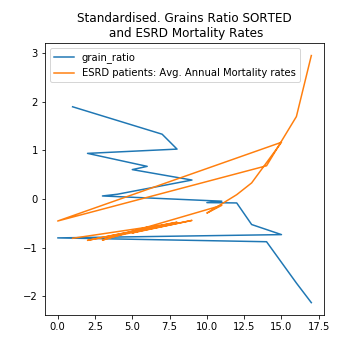
\includegraphics[scale=0.25]{./images/sorted_standard_grain_ratio_negative.png}  }  &  \specialcell{ 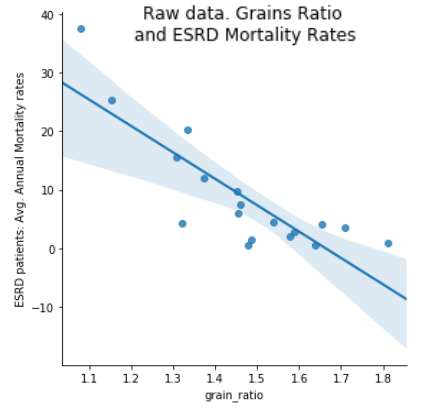
\includegraphics[scale=0.25]{./images/grain_later.png} } \\
Grains & Grains \\
\end{tabular}
\centering
\vspace{0.25cm}
\begin{tabular}{cc}	
\specialcell{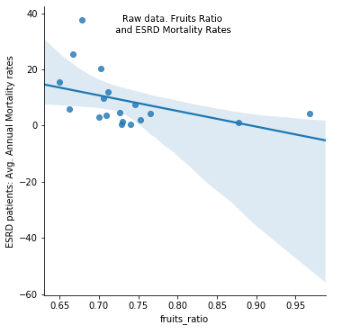
\includegraphics[scale=0.3]{./images/pair_plot_fruits_ratio} } & \specialcell{ 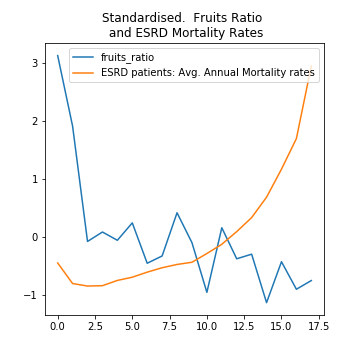
\includegraphics[scale=0.25]{./images/standard_fruit_ratio_mortality.png} } \\
Fruits & Fruits \\
\end{tabular}
\caption{\textbf{Food Groups and Mortality - Negative Correlations}}
\vspace{0.25cm}
\end{figure}

\begin{figure}
\small
\begin{tabular}{cc}	
	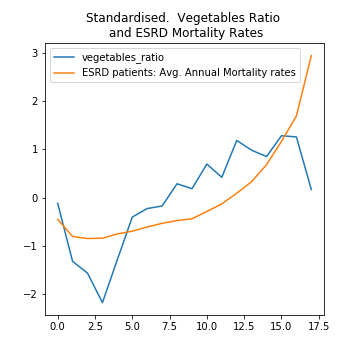
\includegraphics[scale=0.25]{./images/standard_vegetable_ratio.png} & 
	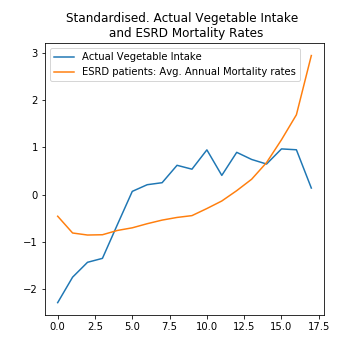
\includegraphics[scale=0.25]{./images/standard_actual_vegetable_intake_esrd_mortality.png}\\
	\multicolumn{2}{c} { 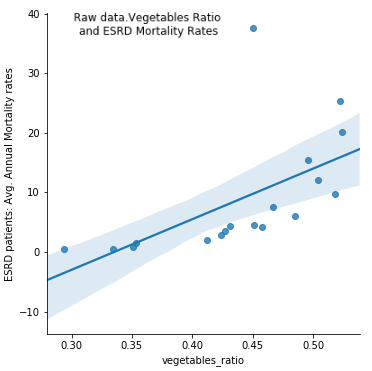
\includegraphics[scale=0.25]{./images/pairplot_vegetable_.png}} 	  \\
	\multicolumn{2}{c}{Vegetables Ratio}  \\ 
\end{tabular}
\centering
\caption{\textbf{Food Groups and Mortality - Positive Correlations (Vegetables) }}
\end{figure}

\noindent Vegetables show positive (0.58) correlation i.e. mortality is high for the patients who took more vegetables. The correlation of 0.58 does not provide a very strong conclusion. Data shows such correlations in older adults. Even though ratios of food intake amount to high end of recommended amounts (actual intake amounts also show positive relation) were used; age might have biased the correlation. This does not show conformity with the general recommendation to take more vegetables for CKD patients. However, as experiments with food subgroups show that vegetable subgroups such as Other vegetables (0.68), Red and Orange vegetables (0.55), and Starchy vegetables (0.44) show positive correlations that have an impact on the Vegetable group correlation.  Although more vegetable intake is a general recommendation for CKD patients, certain vegetables with more carbohydrates (and sugars) such as Starchy Vegetables as well as Vegetables with more Potassium and Calcium such as Tomatoes, and Spinach are recommended to be taken at a lower amount. For diabetes induced CKD, starchy vegetables are not highly recommended in general. Considering the subgroups, the moderate positive correlation as this study found for vegetables food group is in conformity with the general recommendations for CKD patients.

\noindent Experiments (Set 2) with aggregated NHANES and USRDS data to find associations between food subgroups and CKD mortality using PCA and Regression show that  Other vegetables (0.68),    Red and orange vegetables (0.55), and Starchy vegetables (0.44)  have positive correlations with mortality i.e. mortality is low when the intake amounts are low, and mortality is high when intake amounts are high. Data Exploration plots as given below also show these positive relations.

\noindent  Food subgroups such as Alcoholic Beverages (-0.79),    Added Sugars/Sugars and Sweets (-0.64), Whole Grains (-0.61), and  `Nuts, Seeds, and Soy Products' (-0.55) show the most negative correlations with CKD mortality. Data exploration also shows negative correlations as shown in the charts below. These outcomes are also consistent with current knowledge except for Sugars. Prevalence of Stage 3 CKD is lower in Alcohol Drinkers than non-drinkers [2, 49], Nuts being Phosphorus rich and Whole Grains being Potassium rich are detrimental to CKD patients and can cause higher mortality when taken in higher quantities.

\begin{figure}
\small
\begin{tabular}{cc}
	\specialcell{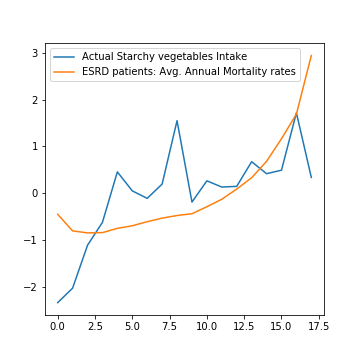
\includegraphics[scale=0.25]{./images/standard_actual_starchy_vegetable_esrd_mortality.png} \\  Starchy Vegetables } & 
	\specialcell{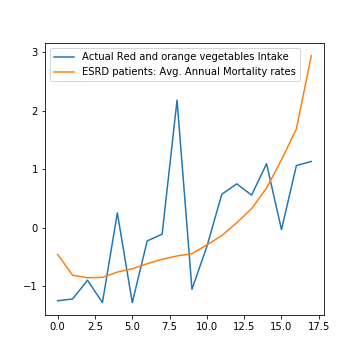
\includegraphics[scale=0.25]{./images/standard_actual_red_and_orange_vegetable_esrd_mortality.png} \\ Red and Orange Vegetables } \\
	 \multicolumn{2}{c} { \specialcell{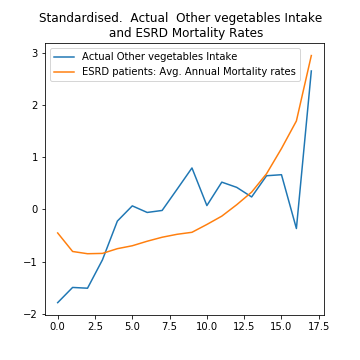
\includegraphics[scale=0.25]{./images/standard_actual_other_vegetable_esrd_mortality.png}	\\ Other Vegetables } } \\
\end{tabular}
\centering
\caption{\textbf{Food Subgroups and Mortality - Positive Correlations}}
\begin{tabular}{cc}
	\specialcell{ 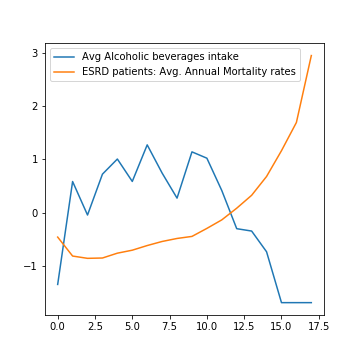
\includegraphics[scale=0.25]{./images/negatively_subgroup_avg_alcohol_intake}  \\   Alcohol Intake  }  & 
	\specialcell{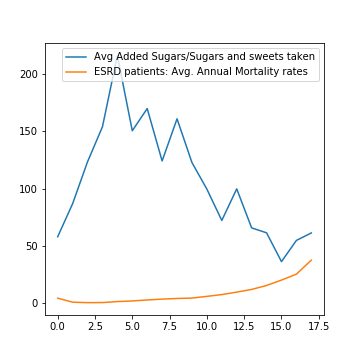
\includegraphics[scale=0.25]{./images/negatively_added_sugar_subgroup_line_2}   \\  Sugar }  \\
	
	\specialcell{ 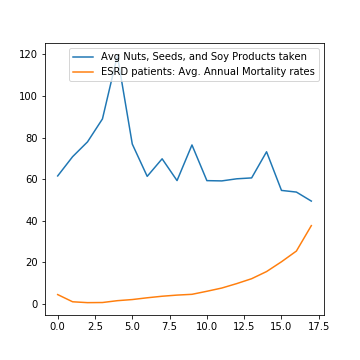
\includegraphics[scale=0.25]{./images/negatively_avg_nuts_subgroup_line_3}  \\ Nuts, Seeds } &
	\specialcell{ 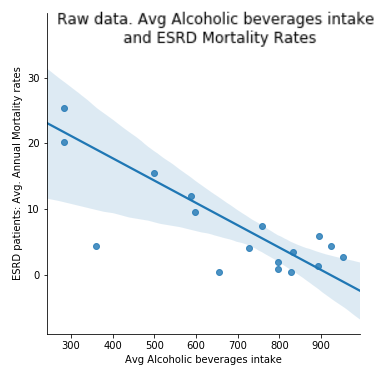
\includegraphics[scale=0.25]{./images/pairplot_avg_alc.png}  \\ Alcohol } \\
	
	\specialcell{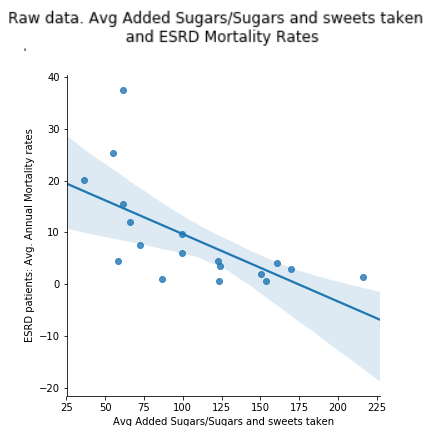
\includegraphics[scale=0.25]{./images/pairplot_raw_data_added_sugar_esrd}  \\ Added Sugar } &
	\specialcell{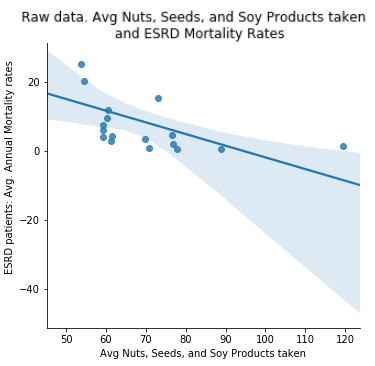
\includegraphics[scale=0.25]{./images/pairplot_nuts_avg_negative.png}  \\ Nuts, Seeds } \\
\end{tabular}
\centering
\caption{\textbf{Food Subgroups and Mortality - Negative Correlations}}
\end{figure}

\noindent \textbf{Mortality Study with Non-aggregated Data}

\noindent For experiments (Set 7) where mortality rates based on ages were used for each NHANES survey row (i.e. not aggregated), the following food subgroups show more positive correlations than others: Fats, Eggs, Other vegetables, Nonalcoholic beverages, White potatoes and Puerto Rican starchy vegetables, Tomatoes and tomato mixtures, Oils, Deep-yellow vegetables respectively. In the study, the following subgroups showed more negative correlations than others: Grain mixtures, Frozen plate meals, Soups, Crackers and Salty snacks from grain products, Milks and milk drinks, Sandwiches with Meat, Poultry, and fish, Poultry. Although the correlation numbers in this study are very low, the positive and negative correlations are consistent with current knowledge [48, 49, 50, 51, 52, 53, 54, 55, 56, 57].


\noindent \textbf{Food Groups, Food Nutrients, and Albumin to Creatinine Ratio (ACR) Association}

\noindent The experiments (Set 3, 4, and 5) using PCA and Regression showed negligible correlation between ACR and food groups and subgroups intake. However, some food groups and/or nutrients such as Dairy, and  `Sugars, Sweets, and Beverages'  have higher and positive though negligible (0.02) effect than the others where Fruits (-0.01) showed negative effect.  For nutrients, Polyunsaturated fatty acids (-0.02), and Iron (-0.02) have negative correlations where Choline (0.02) showed better positive correlation than others. Findings for Choline matches with medical knowledge [48]. As the correlations are not significant further analysis can be done on the data especially for food groups and nutrients that are found important (using PCA) in the data as provided below:

\noindent Dairy,  Fats, oils, and salad dressings’,  Fruits,  Grains,  Protein,   Sugars, sweets, and beverages’, Vegetables, Avg energy kcal,  avg protein gm,  avg carbohydrate gm,  avg total fat gm,  avg total saturated fatty acids gm, avg total monounsaturated fatty acids gm,  avg total polyunsaturated fatty acids gm, avg lutein zeaxanthin mcg,  avg thiamin vitamin B1 mg,  avg riboflavin Vitamin B2 mg,  avg Niacin mg, avg Calcium mg,  avg Phosphorus mg,  avg Magnesium mg,  avg Iron mg, avg Zinc mg,  avg Copper mg,  avg Sodium mg,  avg Potassium mg,  avg Selenium mcg,  Hexadecenoic gm,  Octadecenoic gm

\subsection{Food Subgroups and Albumin to Creatinine Ratio (ACR) Association}

\noindent The experiments showed  `Milk desserts, Sauces, Gravies' (0.22), and Alcoholic Beverages (0.087) have more positive correlations with ACR than the other food subgroups  i.e. taking more of these food subgroups results higher ACR values. Research by Uehara et al. [55] also shows that excessive Alcohol consumption can cause Proteinuria/Albuminuria (high ACR). Nettleton et al. [56] found that high fat dairy can be linked to high ACR values where low-fat dairy is not strongly linked to high ACR values. However, the correlation as this research found is very low. Low values might still explain a correlation where ACR values might depend on other factors in together than only these food subgroups. Fruits and juicy baby foods show negative correlation (-0.04) though not significant i.e. taking high amount does not increase ACR values that matched with current knowledge [57].
\subsection{Relation with Shift Recommendation}

\noindent \noindent \textbf{Recommended Shift:} Include more vegetables from all subgroups where with few exceptions, the U.S. population does not meet intake recommendations for any of the vegetable subgroups. 

\noindent \textbf{Our Study:} This study found moderate positive correlations with mortality for CKD patients. Hence, more vegetables intake is from all vegetable subgroups is not highly recommended  for CKD patients. As this study also finds that food subgroups such as Other Vegetables, Red and Orange Vegetables, and Starchy vegetables are positively correlated with mortality; hence, limiting these subcategories with moderate intake of overall vegetables can be beneficial to CKD patients. 

\noindent\rule{7.8cm}{0.4pt}

\noindent \textbf{Recommended Shift:} Increase fruit (whole fruit) intake for all individuals. Also, take fruits as snacks, salads, and side-dishes.

\noindent \textbf{Our Study:} This study finds Fruits has negative correlations with CKD mortality. Hence, more fruits intake will be beneficial to CKD patients. Shift recommendation is in align with our study.

\noindent\rule{7.8cm}{0.4pt}

\noindent \textbf{Recommended Shift:} Half of all grains should be whole grain.

\noindent \textbf{Our Study:} This study found strong negative correlation of Grains with CKD mortality i.e. more Grain intake showed low mortality rates. Hence, like shift recommendations, CKD patients will benefit by taking recommended amount of Grains. However, this Grain intake includes both whole and refined grain intake. This study also found that Whole grain has moderate negative correlation with mortality i.e. Refined grain contributed to the overall strong correlation. Hence, refined grain-based products can be seen to contribute in negative correlation. Whole grains having rich in Potassium are not highly recommended for CKD patients (I have to check for what level of CKD). CKD patients might get benefit with a mix of whole and refined grain based products where finding the ideal ratio will need further research.

\noindent\rule{7.8cm}{0.4pt}

\noindent \textbf{Recommended Shift:} Increase dairy intake in fat-free form.

\noindent \textbf{Our study:}  This study did not find any strong correlation between dairy products and mortality. However, this study found positive correlation of Urine ACR with dairy products i.e. Urine ACR is high when dairy products are taken more. 

However, the recommended Shift i.e. Increase dairy intake in fat-free form consistent with the recommendation done to CKD patients.

\noindent\rule{7.8cm}{0.4pt}

\noindent \textbf{Recommended Shift:} Increase seafood intake where Teen boys and adult men are recommended to reduce protein intake (instead increase/replace that with vegetables)

\noindent \textbf{Our study:} This study did not find any strong correlation between protein and mortality. 

However, CKD patients based on stages of CKD are recommended to take moderate amount of Protein. The recommended shift i.e. Reduce protein intake for Teen Boys and Adult Men will help CKD patients for that age groups along with others. 

\noindent\rule{7.8cm}{0.4pt}

\noindent \textbf{Recommended Shift:} Increase Oil intake and reduce solid fat intake. Use Oils rather than solid fats.

\noindent \textbf{Our Study:} This study did not see any strong correlation in this regard for CKD patients

\noindent\rule{7.8cm}{0.4pt}

\noindent \textbf{Recommended Shift:} Reduce added sugars to less than 10\% of calories intake per day. 

\noindent \textbf{Our Study:} This study found negative correlation between CKD mortality and Added Sugars i.e. Less sugar intake is related to high mortality. This is contradictory to current knowledge and goes against shift recommendation. However, investigation is required on our data and finding to see what were included in the sugar category. 

\noindent\rule{7.8cm}{0.4pt}

\noindent \textbf{Recommended Shift:} Reduce saturated fat intake to 10\% of calories per day. Shift to take more  polyunsaturated and monounsaturated fats than saturated fats.

\noindent \textbf{Our study:} Polyunsaturated fatty acids have negative correlation with CKD mortality i.e. CKD patients will benefit by taking more  Polyunsaturated fatty acids. Hence, recommended shift will benefit CKD patients.

\noindent\rule{7.8cm}{0.4pt}

\noindent \textbf{Recommended Shift:} Reduce Sodium Intake.

\noindent \textbf{Our Study:} This study did not find any correlation between Sodium and CKD Mortality (I have to verify to what extent sodium is included or not in the study).

\section *{Conclusions}
CKD leading to End Stage Renal Disease is very prevalent today; treatment facilities for dialysis, and donors for organ transplantation are limited. Consequently, many patients die waiting for  proper treatment \cite{Bloomberg2019}. Majority of the studies focused on drugs to control CKD progression where some studies focused on diets, nutrients, and individual food items. Controlling CKD using changes to dietary patterns can be beneficial to both the patients and the economy. Hence, this study focused on the effect of dietary patterns on CKD mortality and a CKD measure named Albumin to Creatinine Ratio (ACR). This study also compared the findings with Dietary Recommendations shift for Impact on CKD patients. PCA and Regression are used to study the association between ACR and CKD mortality/survival. Grains, Fruits, Alcohols, Nuts showed negative correlations where Vegetables such as Other Vegetables, Starchy Vegetables, and Red and Orange Vegetables showed positive correlations. Overall, the results of this research matched the findings of other studies and current knowledge with few exceptions. ACR values were not found strongly correlated with dietary patterns. Comparison with Dietary Recommendations Shift study found that recommended shifts on Fruits, Fats, Polyunsaturated Fats will be beneficial to CKD patients whereas adaptations to reduce harmful effects are required for Vegetables, Whole and Refined Grains.

\makeatother

\section*{Acknowledgments}

%%Vancouver style references.
\bibliographystyle{model3-num-names}
\bibliography{references}

\end{document}
%%
